%%%%%%%%%%%%%%%%%%%%%%%%%%%%%%%%%%%%%%%%%%%%%%%%%%%%%%%%%%%%%%%%%%%
%TO AVOID FORMATTING ISSUES, COMPILE THIS ONLY AT WWW.OVERLEAF.COM%
%%%%%%%%%%%%%%%%%%%%%%%%%%%%%%%%%%%%%%%%%%%%%%%%%%%%%%%%%%%%%%%%%%%
%AUTHOR: 
%CLASS:  
%%%%%%%%%%%%%%%%%%%%%%%%%%%%%%%%%%%%%%%%%%%%%%%%%%%%%%%%%%%%%%%%%%%
\documentclass[a4paper,12pt]{article}
\usepackage{graphicx}
\newenvironment{codeblock}{\fontfamily{pcr}\selectfont}{\par}

\title{
	\normalfont \normalsize 
	\textsc{Pimpri Chinchwad College of Engineering \\ 
		Computer Laboratory - III} \\
	[10pt] 
	\rule{\linewidth}{0.5pt} \\[6pt] 
	\huge Assignment No - 4 \\
	\rule{\linewidth}{2pt}  \\[10pt]
}
\author{}
\date{\normalsize}


\begin{document}
\maketitle

%%%%%%%%%%%%%%%%%%%%%%%
% FOR A NUMBERED LIST
% \begin{enumerate}
% \item Your_Item
% \end{enumerate}
%%%%%%%%%%%%%%%%%%%%%%%
% FOR A BULLETED LIST
% \begin{itemize}
% \item Your_Item
% \end{itemize}
%%%%%%%%%%%%%%%%%%%%%%%
% TO IMPORT AN IMAGE
% \includegraphics[width=\textwidth]{name_of_file}
% \textwidth makes the picture the width of the paragraphs
%%%%%%%%%%%%%%%%%%%%%%%%%%%%%%
% TO CREATE A FIGURE WITH A NUMBER AND CAPTION
% \begin{figure}
% \includegraphics[width=\textwidth]{image}
% \caption{Your Caption Goes Here}
% \label{your_label}
% \end{figure}
% REFER TO YOUR FIGURE LATER WITH
% \ref{your_label}
% LABELS NEED TO BE ONE WORD
%%%%%%%%%%%%%%%%%%%%%%%%%%%%%
% TO ADD CODE
% \begin{codeblock}
% Some code in "courier" font
%\end{codeblock}
%%%%%%%%%%%%%%%%%%%%%%%%%%%%%
\section{Aim}
	\paragraph{} Produce a DSA signature using parameter tuple \{p,q,g\}, long term key pair and a message digest
	
\section{Objective}
	\begin{itemize}
		\item To understand working of Digital Signature Algorithm generator.
		\item To generate public and private key for signing message
        \item To generate message digest from source message
        \item To sign the message digest using private key
        \item To verify the authenticity of digital signature using public key
	\end{itemize}
	
\section{Software Requirements}
	\begin{itemize}
		\item	Linux Operating System
		\item	C++
	\end{itemize}
	
\section{Mathematical Model}
\paragraph{} 
S 	= {s, e, x, y, Fme, DD, NDD}  											\\\\
S   =   Initial State  										\\
E 	=   End State  																\\
X	= Input Value\\
X=\{x1,x2, x3\} \\
where,  x1=p\\
x2=q\\
x3=plaintext message\\
Y	=Output\\
Y=\{y1,y2\}\\
y1=\{"Public Key"\}\\
y2=\{"Private Key"\}\\
Fme 	= 	Main function \\
Fme=\{f1\}\\f1="DSA Algorithm to perform data encryption".\\
Pu=DSA(x3)\\
Pr=DSA(x3)\\
where, Pu = Pubic Key.\\
Pr = Private Key.\\
DD 	= 	Deterministic data \{plaintext\}\\
NDD	= 	Non Deterministic Data \{public key, private key\}			\\
	
		
	
\section{Theory}
	\paragraph{} A digital signature algorithm (DSA) refers to a standard for digital signatures. It was introduced in 1991 by the National Institute of Standards and Technology (NIST) as a better method of creating digital signatures. Along with RSA, DSA is considered one of the most preferred digital signature algorithms used today.
    \paragraph{} Unlike DSA, most digital signature types are generated by signing message digests with the private key of the originator. This creates a digital thumbprint of the data. Since just the message digest is signed, the signature is generally much smaller compared to the data that was signed. As a result, digital signatures impose less load on processors at the time of signing execution, use small volumes of bandwidth, and generate small volumes of ciphertext intended for cryptanalysis.
    \paragraph{} DSA, on the other hand, does not encrypt message digests using private key or decrypt message digests using public key. Instead, it uses unique mathematical functions to create a digital signature consisting of two 160-bit numbers, which are originated from the message digests and the private key. DSAs make use of the public key for authenticating the signature, but the authentication process is more complicated when compared with RSA.
    \paragraph{} The digital signature procedures for RSA and DSA are usually regarded as being equal in strength. Because DSAs are exclusively used for digital signatures and make no provisions for encrypting data, it is typically not subject to import or export restrictions, which are often enforced on RSA cryptography.
			
\section{Algorithm}
	\paragraph{Parame Generation:} The first part of the DSA algorithm is the public key and private key generation, which can be described as: 
    \begin{codeblock}
    \begin{enumerate}
        \item Choose a prime number q, which is called the prime divisor.
        \item Choose another primer number p, such that p-1 mod q = 0. p is called the prime modulus.
        \item Choose an integer g, such that 1 < g < p, $g^{q}$ mod p = 1 and g = $h^{(p–1)/q)} mod p$. q is also called g's multiplicative order modulo p.
        \item Choose an integer, such that 0 < x < q.
    Compute y as $g^{x}$ mod p.
    	\item Package the public key as {p,q,g,y}.
    Package the private key as {p,q,g,x}.
	\end{enumerate}
    \end{codeblock}

     \begin{figure}
     	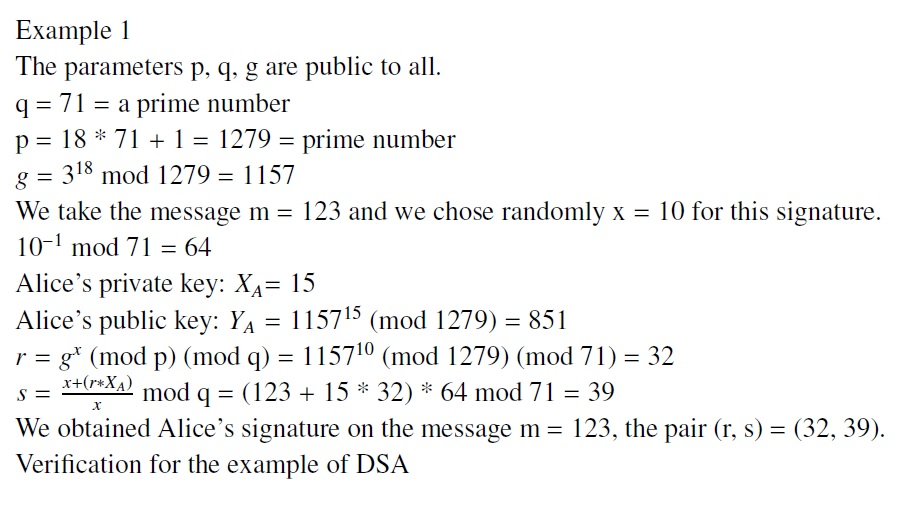
\includegraphics[width=\textwidth]{dsa}
     	\caption{Example 1}
     \end{figure}
    
    
    \paragraph{Signature Generation and Verification:} The second part of the DSA algorithm is the signature generation and signature verification, which can be described as:

To \textbf{generate} a message signature, the sender can follow these steps: 
	\begin{codeblock}
	\begin{enumerate}
    	\item Generate the message digest h, using a hash algorithm like SHA1.
    	\item Generate a random number k, such that 0 < k < q.
    	\item Compute r as ($g^{k}$ mod p) mod q. If r = 0, select a different k.
    	\item Compute i, such that k*i mod q = 1. i is called the modular multiplicative inverse of k modulo q.
    	\item Compute s = i*(h+r*x) mod q. If s = 0, select a different k.
    	\item Package the digital signature as {r,s}.
	\end{enumerate}
    \end{codeblock}
    
    
To find multiplicative inverse: 
	\begin{codeblock}
	\begin{verbatim}
	    
	
    	ExtEuclid (a,b) {
   // returns a triple (d,s,t) such that d = gcd(a,b) and
   // d == a*s + b*t

   if (b == 0) return (a,1,0) ;
   
   (d1, s1, t1) = ExtEuclid(b,a%b) ;
   d = d1 ;
   s = t1 ;
   t = s1 - (a div b) * t1 ;   // note: div = integer division
   return (d,s,t) ;
    }
    \end{verbatim}
    \end{codeblock}
    
To \textbf{verify} a message signature, the receiver of the message and the digital signature can follow these steps: 
	\begin{codeblock}
    \begin{enumerate}	
    	\item Generate the message digest h, using the same hash algorithm.
    	\item Compute w, such that s*w mod q = 1. w is called the modular multiplicative inverse of s modulo q.
    	\item Compute u1 = h*w mod q.
    	\item Compute u2 = r*w mod q.
    	\item Compute v = ((($g^{u1}$)*($y^{u2}$)) mod p) mod q.
    	\item If v == r, the digital signature is valid.
	\end{enumerate}
    \end{codeblock}
    
\section{Conclusion}
	\paragraph{} Thus, we have studied and implemented  DSA signature using parameter tuple \{p,q,g\}, long term key pair and a message digest.
	
\vspace{20px}
\begin{center}
	\begin{tabular}
		{|c|c|c|c|}\hline
		{\bf Roll No.}		&{\bf Name of Student}		&{\bf Date of Performance}  				&{\bf Date of Submission}  \\ \hline
		{302}	&	{Abhinav Bakshi}& {04/02/2016}	&  {18/02/2016} \\ \hline
	\end{tabular}\\ 
\end{center}

\section{Plagarism Report}
  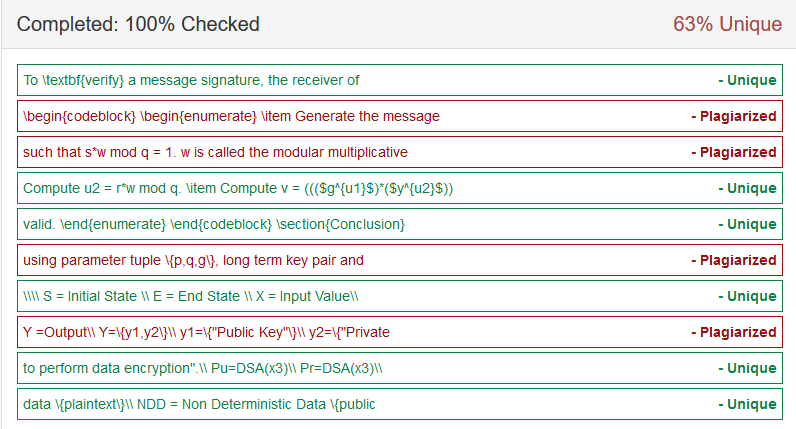
\includegraphics[width=\textwidth]{dsapl}
\section{Output}
\begin{verbatim}
--------------------------------------------
DSA output

Generation
Parameters : 
p : 1279
q : 71
g : 1157

Signing
r : 32
s : 39

Verification

*****Signature Verified*****

*****Signature Verified*****

-------------------------------------------
\end{verbatim}
\end{document}
 

 
